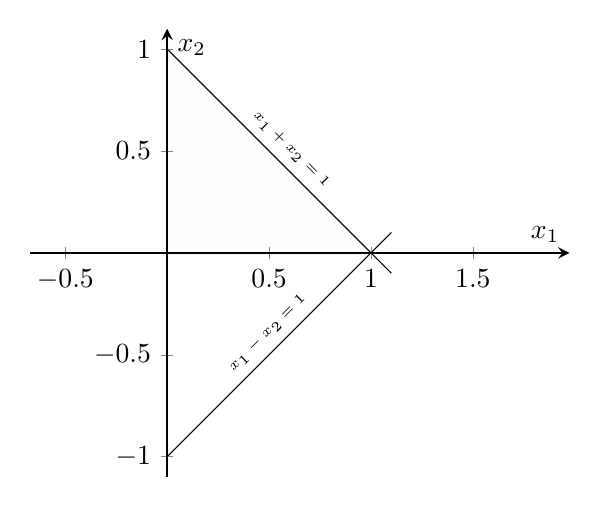
\begin{tikzpicture}
  \begin{axis}[
      xlabel={$x_1$},
      ylabel={$x_2$},
      axis on top=true,
      axis equal,
      axis lines=middle,
      samples=41,
      thick,
      xmin=-0.1,
      xmax=1.4,
      ymin=-1.1,
      ymax=1.1,
]
    \addplot[
      thick,
      color=gray!20,
      fill=gray!20, 
      fill opacity=0.05
    ] coordinates {
      (0, 1) 
      (1, 0)
      (0, 0)
    };
    
    \addplot[
      color=black,
      thin,
      domain=0:1.1
    ] {1 - x}  node[pos=0.5, sloped, above] {\tiny $x_1+x_2=1$};

    \addplot[
      color=black,
      thin,
      domain=0:1.1
    ] {x - 1} node[pos=0.5, sloped, above] {\tiny $x_1-x_2=1$};
  \end{axis}
\end{tikzpicture}
